\documentclass{beamer}
\usepackage{color}
\usepackage{booktabs}
\usepackage{multirow}
\usepackage{amssymb,graphicx}
\usepackage{pifont}

\begin{document}

\title{Multi-UAV Simulation Presentation}   
\author{Srijit Dutta\\} 
\date{\today} 


\frame{\titlepage} 
\section{Report} 



\subsection{Box2D}
\frame{\frametitle{Improvement from previous simulation} 
\begin{itemize}
\item A 2-D model has been developed, this is based on the assumption that the height is constant for all UAVs
\item All UAVs keep monitoring all fires upto a time the 'false alarm' is detected
\item This false alarm is selected randomly and the UAVs adjust their course accordingly
\item Also self collisions among UAVs have been neglected
\end{itemize}
}
%%%%%%%%%%%%%%%%%%%
\frame{\frametitle{Continued..} 
\begin{itemize}
\item The path-planning algorithm discussed last time has been modified a little
\item The priority of the fires/cells are based on the "age"/time it has been unattended for 
\item This makes sure no fire is neglected for a long time
\item Also the parameter of distance in the original algorithm has been replaced by moving to the next unattended fire
\item This does not create a problem when path of 2 UAVs cross
\end{itemize}
}

%%%%%%%%%%%%%%%%%%%%%%%%%%
\frame{\frametitle{Simulation} 
\begin{itemize}
\item The UAVs return to their base station after fire monitoring
\end{itemize}

\begin{figure}[h!]
\centering
 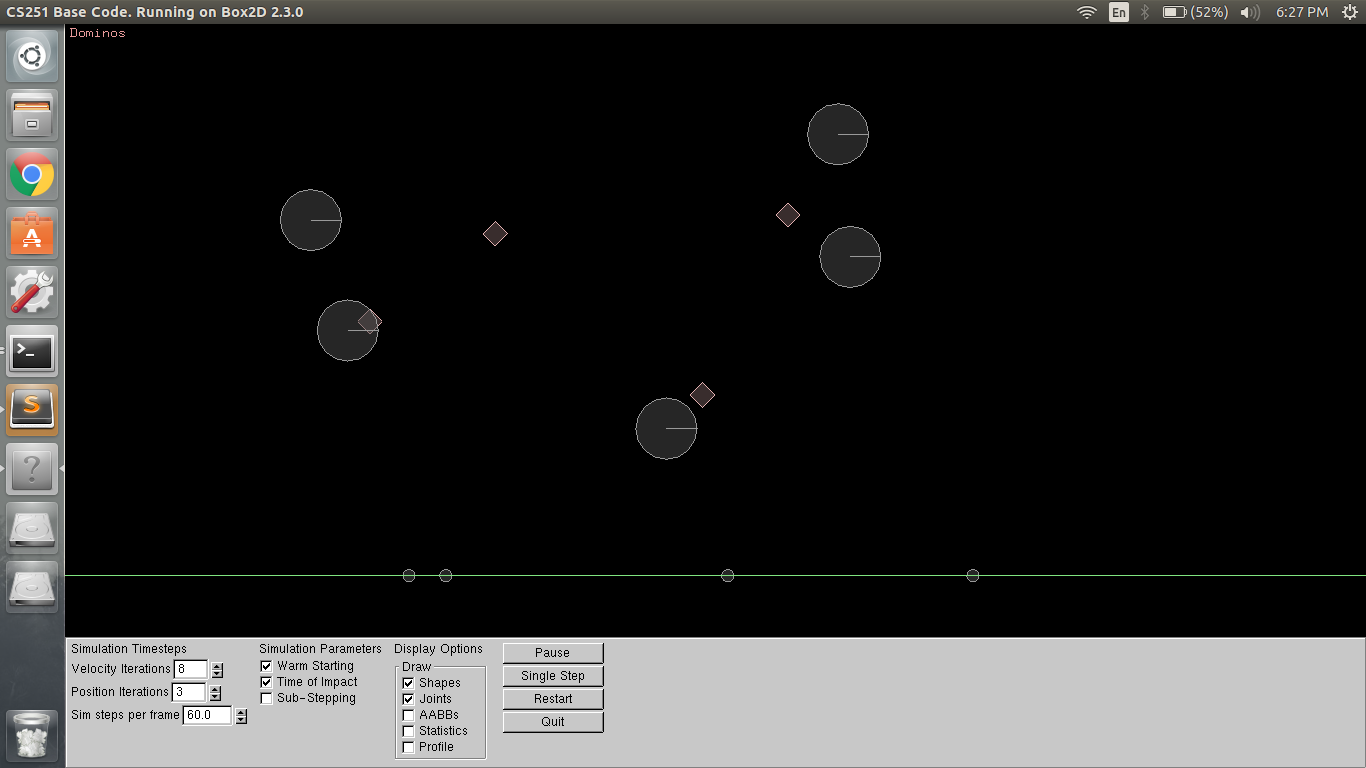
\includegraphics[width=80mm]{motion1.png}
 \caption{Monitoring}
 \label{fig:boat1}
\end{figure}
}

%%%%%%%%%%%%%%%%%%%%%%%%%
\frame{\frametitle{Simulation} 
\begin{itemize}
\item Path planning is adjusted once false fire is detected
\end{itemize}

\begin{figure}[h!]
\centering
 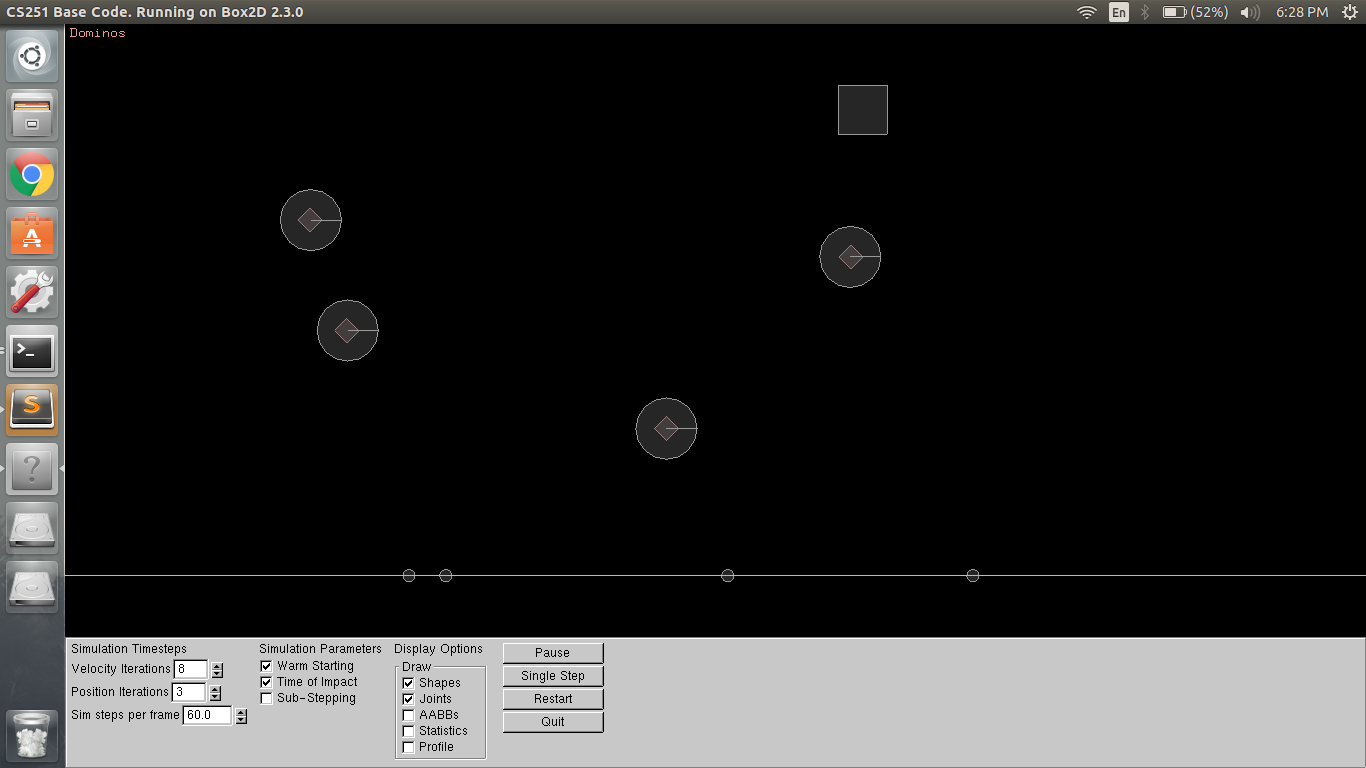
\includegraphics[width=80mm]{fixed1.png}
 \caption{New Arrangement}
 \label{fig:boat2}
\end{figure}
}

\end{document}